\section{内点法}
\label{sec:opt-con-interior-point}

活动集法与SQP都要判断哪些不等式在最优点活跃，这个组合选择在约束很多时可能代价很高。\term{内点法}（interior-point method）换了一个角度：始终待在不等式约束严格成立的内部，用一个在边界处趋于无穷的障碍项阻止迭代越界，再逐步减弱障碍，让迭代沿一条光滑曲线滑向最优点。本节先在线性规划上建立这条曲线——中心路径，然后区分两种沿路径前进的方法：先固定障碍参数把子问题解好再减小参数的障碍法，以及把原始与对偶变量放在一起作牛顿更新的原始—对偶内点法。本节用$\mu>0$表示障碍参数（与强凸常数无关），标准型线性规划$\min\bm c^\top\bm x$、$\bm A\bm x=\bm b$、$\bm x\geq\bm0$中$\bm A\in\mathbb R^{m\times n}$，变量个数为$n$。

\subsection{障碍函数与中心路径}
\label{sec:opt-con-central-path}

\paragraph{对数障碍}
不等式$x_j\geq0$要求迭代不能越过$x_j=0$。若在目标中加入$-\mu\log x_j$，它在$x_j\downarrow0$时趋于$+\infty$，迭代就不会碰到边界；$\mu$越小，障碍对内部的影响越弱。对满行秩的标准型线性规划，构造\term{对数障碍函数}（logarithmic barrier function）问题
\begin{equation}
\label{eq:opt-con-barrier-lp}
  \min_{\bm x}\ B_\mu(\bm x)=\bm c^\top\bm x-\mu\sum_{j=1}^n\log x_j\quad\text{s.t.}\quad\bm A\bm x=\bm b,\ \bm x>\bm0.
\end{equation}
等式约束仍原样保留。$-\log$严格凸，所以$B_\mu$在可行集上严格凸，最小点若存在则唯一。存在性却不是自动的，它需要原始和对偶两侧都严格可行。

\begin{theorem}[中心点的存在唯一]
\label{thm:opt-con-central-path}
设$\bm A$行满秩，存在$\bm x>\bm0$使$\bm A\bm x=\bm b$（原始严格可行），并存在$\bar{\bm y}$与$\bar{\bm s}>\bm0$使$\bm A^\top\bar{\bm y}+\bar{\bm s}=\bm c$（对偶严格可行）。则对每个$\mu>0$，问题~\eqref{eq:opt-con-barrier-lp}有唯一最小点$\bm x(\mu)$。
\end{theorem}

\begin{proof}
在可行集上，$\bm c^\top\bm x=(\bm A^\top\bar{\bm y}+\bar{\bm s})^\top\bm x=\bm b^\top\bar{\bm y}+\bar{\bm s}^\top\bm x$，于是$B_\mu(\bm x)=\bm b^\top\bar{\bm y}+\sum_j\bigl(\bar s_jx_j-\mu\log x_j\bigr)$。每一项$\bar s_jx_j-\mu\log x_j$在$x_j>0$上有下界$\mu-\mu\log(\mu/\bar s_j)$，并在$x_j\downarrow0$或$x_j\to\infty$时趋于$+\infty$。因此对任意可行$\bm x_0>\bm0$，下水平集$\{\bm x:\bm A\bm x=\bm b,\ \bm x>\bm0,\ B_\mu(\bm x)\leq B_\mu(\bm x_0)\}$中每个坐标都被限制在某个$[\epsilon,M]$内（$\epsilon>0$），它是非空紧集。连续函数在其上达到最小，这就是全局最小点；严格凸性给出唯一性。
\end{proof}

对偶严格可行不能省去。$\min0$、约束$x_1-x_2=0$、$\bm x\geq\bm0$的原问题严格可行，最优值为$0$；但$B_\mu=-\mu\log x_1-\mu\log x_2$沿可行射线$x_1=x_2=s\to\infty$趋于$-\infty$，没有最小点。它的对偶约束$y\leq0$、$-y\leq0$迫使$y=0$、$\bm s=\bm0$，没有严格可行的对偶点。只凭原始严格可行和有限最优值，不能宣称中心路径存在。

\paragraph{中心路径与间隙}
最小点由KKT条件刻画：存在$\bm y$使$\bm c-\mu\bm X^{-1}\bm1-\bm A^\top\bm y=\bm0$，其中$\bm X=\operatorname{diag}(\bm x)$。令$\bm s=\mu\bm X^{-1}\bm1>\bm0$，条件变为
\begin{equation}
\label{eq:opt-con-central-path}
  \bm A\bm x=\bm b,\quad\bm A^\top\bm y+\bm s=\bm c,\quad x_js_j=\mu\ (j=1,\dots,n),\quad\bm x,\bm s>\bm0.
\end{equation}
与线性规划的KKT条件对照，前两组是原始与对偶可行性，第三组本应是互补松弛$x_js_j=0$，现在被“扰动”为$x_js_j=\mu$。当$\mu$从$+\infty$减小到$0$，解$(\bm x(\mu),\bm y(\mu),\bm s(\mu))$画出一条曲线，称为\term{中心路径}（central path）。沿这条路径，原始—对偶间隙可以精确算出：
\[
  \bm c^\top\bm x(\mu)-\bm b^\top\bm y(\mu)=(\bm A^\top\bm y+\bm s)^\top\bm x-(\bm A\bm x)^\top\bm y=\bm s^\top\bm x=n\mu.
\]
$\bm x(\mu)$原始可行，$\bm y(\mu)$对偶可行，由弱对偶，$\bm x(\mu)$的次优性不超过$n\mu$。要得到$\epsilon$精度，只需走到$\mu\leq\epsilon/n$。这个界成立的前提是精确位于中心点；迭代只是近似中心时，还要计入离中心的偏差和内层求解误差。

\begin{example}[两变量的中心路径]
\label{ex:opt-con-central-path}
$\min x_1+2x_2$、$x_1+x_2=1$、$\bm x\geq\bm0$，最优点$(1,0)^\top$，对偶最优$y^\star=1$。由式~\eqref{eq:opt-con-central-path}，$x_j=\mu/(c_j-y)$，代入$x_1+x_2=1$得$\mu(3-2y)=(1-y)(2-y)$。取满足$y<1$的根，$y(\mu)=\bigl(3-2\mu-\sqrt{4\mu^2+1}\bigr)/2$。$\mu=1$时$y\approx-0.618$，$\bm x\approx(0.618,0.382)^\top$，间隙$x_1+2x_2-y=2$；$\mu=0.1$时$y\approx0.890$，$\bm x\approx(0.910,0.090)^\top$，间隙$0.2$。两次都等于$n\mu=2\mu$。$\mu\to0$时$y\to1$、$\bm x\to(1,0)^\top$。
\end{example}

图~\ref{fig:opt-con-central-path}把同一构造放到三个变量上：$\min x_1+2x_2+3x_3$，$x_1+x_2+x_3=1$。可行域是单纯形，画成三角形。$\mu$很大时障碍项主导，中心点接近三角形的重心（解析中心）；$\mu$减小时，中心点沿一条光滑曲线移向最优顶点$\bm e_1$，始终不碰边界。绿色曲线是$\mu=0.3$时障碍目标的等值线：它们在边界附近陡然升高，在内部围出一个“碗”，碗底就是$\bm x(0.3)\approx(0.670,0.207,0.123)^\top$。

\begin{figure}[!htbp]
  \centering
  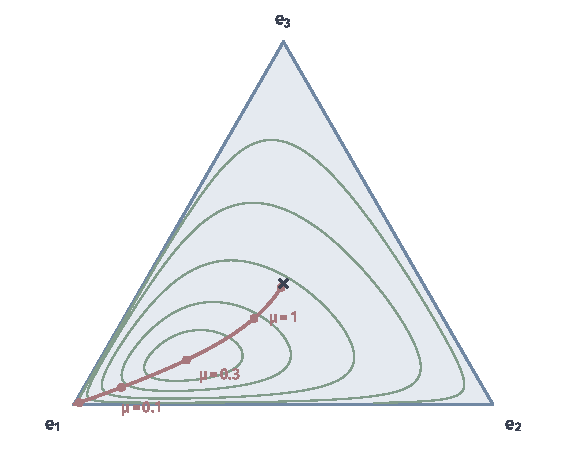
\includegraphics[width=96mm]{figures/03-optimization-evolution-and-signals/01-optimization/matplotlib/c5-central-path/figure.pdf}
  \caption{$\min x_1+2x_2+3x_3$、$x_1+x_2+x_3=1$、$\bm x\geq\bm0$的中心路径，单纯形用重心坐标画成三角形。红色曲线为$\mu$从$10^3$减小到$10^{-3}$的中心点$\bm x(\mu)$，从重心附近（黑叉）出发通向最优顶点$\bm e_1$；红点标出$\mu=10,1,0.3,0.1,0.01$，对应间隙$3\mu$。绿色曲线为$\mu=0.3$时障碍目标$B_\mu$的等值线。}
  \label{fig:opt-con-central-path}
\end{figure}

\subsection{障碍法}
\label{sec:opt-con-barrier-method}

\paragraph{外层减小参数，内层牛顿居中}
\term{障碍法}（barrier method）沿中心路径分段前进：固定$\mu$，用牛顿法把问题~\eqref{eq:opt-con-barrier-lp}解到足够接近中心点；然后把$\mu$缩小一个固定比例，以当前点为热启动，重复。$B_\mu$的梯度为$\bm c-\mu\bm X^{-1}\bm1$，Hessian为$\mu\bm X^{-2}$。在等式约束$\bm A\bm x=\bm b$下，牛顿步$\Delta\bm x$保持$\bm A\Delta\bm x=\bm0$，由线性系统
\[
  \begin{bmatrix}\mu\bm X^{-2}&\bm A^\top\\\bm A&\bm0\end{bmatrix}
  \begin{bmatrix}\Delta\bm x\\\bm w\end{bmatrix}
  =\begin{bmatrix}-(\bm c-\mu\bm X^{-1}\bm1)\\\bm0\end{bmatrix}
\]
确定，这是第~\ref{chap:opt-smooth}章牛顿法加上等式约束的形式，系数矩阵就是式~\eqref{eq:opt-con-kkt-matrix}的KKT矩阵。步长要保持$\bm x>\bm0$：先取使$\bm x+\alpha\Delta\bm x>\bm0$的最大$\alpha$乘以$0.99$之类的系数，再在$B_\mu$上作回溯线搜索。

\begin{algorithm}[障碍法（标准型线性规划）]
\label{alg:opt-con-barrier}
\begin{algorithmic}[1]
\Require 严格可行初值$\bm x>\bm0$（$\bm A\bm x=\bm b$），$\mu_0>0$，缩小因子$\theta\in(0,1)$，精度$\epsilon$，居中容差
\Ensure 近似最优点$\bm x$
\Loop
  \Repeat\Comment{居中：牛顿法求$B_\mu$的最小点}
    \State 解上面的KKT系统得$\Delta\bm x$；取保持$\bm x>\bm0$的步长并在$B_\mu$上回溯；更新$\bm x$
  \Until{牛顿减量$(\Delta\bm x^\top\mu\bm X^{-2}\Delta\bm x)^{1/2}$低于居中容差}
  \If{$n\mu\leq\epsilon$}
    \State 返回$\bm x$
  \EndIf
  \State $\mu\leftarrow\theta\mu$
\EndLoop
\end{algorithmic}
\end{algorithm}

\paragraph{起点与可行性阶段}
算法需要一个严格可行的起点。没有现成的起点时，先求解一个辅助问题，例如$\min_{\bm x,\sigma}\sigma$、$\bm A\bm x=\bm b$、$x_j+\sigma\geq0$：取任意满足$\bm A\bm x=\bm b$的$\bm x$和足够大的$\sigma$，它就是辅助问题的严格可行点。辅助问题的最优值$\sigma^\star<0$时，得到严格可行的起点；$\sigma^\star>0$时，原问题不可行；$\sigma^\star=0$时，原问题可行但没有严格可行点，不满足本节的假设，需要先消去恒为零的变量再处理。这一区分很重要：“原问题不可行”与“可行但不满足严格可行假设”需要不同的报告。

\paragraph{停止、成本与数值问题}
停止由两部分共同决定：外层的$n\mu\leq\epsilon$控制中心点的间隙，居中容差控制当前点离中心点多远。外层迭代次数约为$\log(n\mu_0/\epsilon)/\log(1/\theta)$；每次外层的牛顿步数取决于$\theta$：缩得越猛，外层越少，但每次居中需要的牛顿步越多。每个牛顿步的主要成本是解KKT系统，常消去$\Delta\bm x$得到$m\times m$的正规方程$\bm A\bm X^2\bm A^\top\bm w=\cdots$，稠密时形成需$O(m^2n)$、分解需$O(m^3)$，稀疏时取决于$\bm A$的结构。这三者——外层次数、每次的牛顿步数、每步的线性求解——应分开计量。

利用障碍函数的自协调性质，可以证明短步长的路径跟踪方法至多需要$O(\sqrt n\log(n\mu_0/\epsilon))$次牛顿步\scite{math-boyd2004convex}；这一理论的细节作为补充，不在此展开。实践中观察到的外层次数往往很少，但这只是经验，不能当作统一的成本界。另一个实际问题是数值病态：接近最优点时，最优解为零的那些坐标$x_j\to0$，$\mu\bm X^{-2}$的对应元素约为$s_j^2/\mu\to\infty$，而另一些元素趋于零，KKT系统的条件数随之恶化。成熟的实现依靠专门的分解与正则化处理这一问题，用户至少应检查最终残差，而不是只看算法是否报告收敛。

\paragraph{推广到二阶锥与半正定约束}
同样的思路适用于第~\ref{sec:opt-con-quadratic-conic}节的锥模型，只需换一个在锥内部有定义、在边界处趋于无穷的障碍。二阶锥$\{(\bm u,t):\lVert\bm u\rVert_2\leq t\}$的内部是$t>\lVert\bm u\rVert_2$，取$-\log(t^2-\lVert\bm u\rVert_2^2)$；半正定锥的内部是$\bm X\succ\bm0$，取$-\log\det\bm X$，它的梯度为$-\bm X^{-1}$，Hessian作用在方向$\bm D$上为$\bm X^{-1}\bm D\bm X^{-1}$。中心路径上的间隙不再是变量个数乘$\mu$，而是由障碍决定的常数乘$\mu$：每个二阶锥贡献$2\mu$，每个$k\times k$半正定块贡献$k\mu$（在中心点$\bm X\bm S=\mu\bm I$，间隙$\operatorname{tr}(\bm X\bm S)=k\mu$），所以不能照搬线性规划的$n\mu$。计算上的主要变化在牛顿系统：半正定规划中形成$m\times m$的系数矩阵需要计算$\operatorname{tr}(\bm A_i\bm X\bm A_l\bm X)$，稠密时代价约为$O(mk^3+m^2k^2)$，存储也从向量变为$k\times k$矩阵；问题规模较大时，这往往是半正定规划的瓶颈。

\subsection{原始—对偶内点法}
\label{sec:opt-con-primal-dual-ipm}

\paragraph{对扰动的KKT方程组作牛顿法}
障碍法只把$\bm x$当作迭代变量，乘子是居中后才读出的。另一种做法直接把式~\eqref{eq:opt-con-central-path}看作关于$(\bm x,\bm y,\bm s)$的非线性方程组，并且不必等居中完成就降低目标$\mu$。在当前点$(\bm x,\bm y,\bm s)$（$\bm x,\bm s>\bm0$，不要求满足等式）处，记$\bm r_{\mathrm p}=\bm A\bm x-\bm b$、$\bm r_{\mathrm d}=\bm A^\top\bm y+\bm s-\bm c$、平均互补量$\bar\mu=\bm x^\top\bm s/n$，目标参数取$\sigma\bar\mu$（$\sigma\in(0,1)$），对方程组作牛顿线性化：
\begin{equation}
\label{eq:opt-con-pd-newton}
  \begin{bmatrix}\bm0&\bm A^\top&\bm I\\\bm A&\bm0&\bm0\\\bm S&\bm0&\bm X\end{bmatrix}
  \begin{bmatrix}\Delta\bm x\\\Delta\bm y\\\Delta\bm s\end{bmatrix}
  =-\begin{bmatrix}\bm r_{\mathrm d}\\\bm r_{\mathrm p}\\\bm X\bm S\bm1-\sigma\bar\mu\bm1\end{bmatrix},
\end{equation}
其中$\bm S=\operatorname{diag}(\bm s)$。前两行是线性方程，第三行线性化了$x_js_j=\sigma\bar\mu$。步长取保持$\bm x,\bm s$严格为正的最大步长乘以$0.99$（不超过$1$），原始与对偶变量同步更新。这就是\term{原始—对偶内点法}（primal-dual interior-point method）。与障碍法“先固定参数求中心点，再减小参数”相比，它每轮只走一步牛顿步，就同时改进可行性、互补性和中心性。

\begin{algorithm}[原始—对偶路径跟踪]
\label{alg:opt-con-primal-dual}
\begin{algorithmic}[1]
\Require $(\bm x,\bm y,\bm s)$，$\bm x,\bm s>\bm0$；居中参数$\sigma\in(0,1)$；容差$\epsilon_{\mathrm p},\epsilon_{\mathrm d},\epsilon_{\mathrm g}$
\Ensure 近似原始—对偶最优三元组
\Repeat
  \State 计算$\bm r_{\mathrm p}$、$\bm r_{\mathrm d}$、$\bar\mu=\bm x^\top\bm s/n$
  \State 解式~\eqref{eq:opt-con-pd-newton}得$(\Delta\bm x,\Delta\bm y,\Delta\bm s)$
  \State $\alpha=\min\{1,\ 0.99\cdot\max\{\alpha':\bm x+\alpha'\Delta\bm x\geq\bm0,\ \bm s+\alpha'\Delta\bm s\geq\bm0\}\}$
  \State $(\bm x,\bm y,\bm s)\leftarrow(\bm x,\bm y,\bm s)+\alpha(\Delta\bm x,\Delta\bm y,\Delta\bm s)$
\Until{$\lVert\bm r_{\mathrm p}\rVert\leq\epsilon_{\mathrm p}$，$\lVert\bm r_{\mathrm d}\rVert\leq\epsilon_{\mathrm d}$，$\bm x^\top\bm s\leq\epsilon_{\mathrm g}$}
\end{algorithmic}
\end{algorithm}

\paragraph{三项残差共同决定停止}
图~\ref{fig:opt-con-pdipm}在一个资源分配线性规划上运行算法~\ref{alg:opt-con-primal-dual}。原问题为$\max3x_1+2x_2$、$2x_1+x_2\leq4$、$x_1+2x_2\leq4$，加入松弛变量化为标准型$\min-3x_1-2x_2$，$n=4$、$m=2$，最优值$-20/3$，最优点$(4/3,4/3,0,0)^\top$。起点取$\bm x=2\cdot\bm1$（不满足等式约束）、$\bm s=\bm1$、$\bm y=\bm0$，$\sigma=0.2$。第一步的步长受正性限制小于$1$，原始残差从$5.66$降到$0.47$；第二步取到全步长，由于前两行是线性方程，原始与对偶残差一步降到舍入误差水平，此后保持可行。互补量$\bm x^\top\bm s$则每步约缩小为原来的$1/5$，从$8$降到第9步的$7\times10^{-6}$。

\begin{figure}[!htbp]
  \centering
  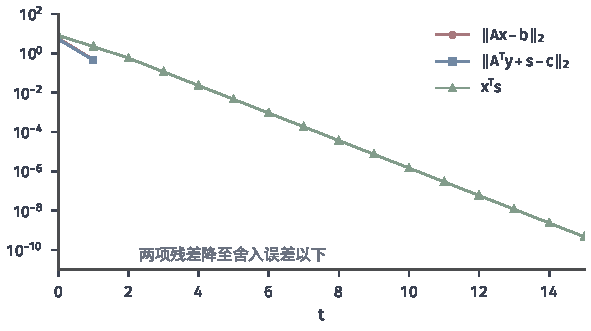
\includegraphics[width=100mm]{figures/03-optimization-evolution-and-signals/01-optimization/matplotlib/c5-pdipm/figure.pdf}
  \caption{一个资源分配线性规划（标准型$n=4$、$m=2$）上的原始—对偶内点法，$\sigma=0.2$，起点$\bm x=2\cdot\bm1$、$\bm s=\bm1$、$\bm y=\bm0$，对数纵轴。红色为原始残差$\lVert\bm A\bm x-\bm b\rVert_2$，蓝色为对偶残差$\lVert\bm A^\top\bm y+\bm s-\bm c\rVert_2$，两者在第2步取全步长后降到$10^{-12}$以下（图中不再画出）；绿色为互补量$\bm x^\top\bm s$，按约$\sigma$的比率几何下降。}
  \label{fig:opt-con-pdipm}
\end{figure}

这个例子也说明为什么三项残差都要监测。第1步后$\bm c^\top\bm x\approx-6.88$，已经低于最优值$-6.67$，因为此时$\bm x$还不满足等式约束；只看互补量或目标值会误判。只有在原始与对偶残差都足够小时，$\bm x^\top\bm s$才近似等于原始—对偶间隙$\bm c^\top\bm x-\bm b^\top\bm y$，才能作为目标误差的证书；两侧都不可行时，互补量单独不是任何误差的上界。实际报告应同时给出三项残差及所用的尺度。

改进方向选择的一种常见做法是预测—校正：先解一次$\sigma=0$的方程组（预测步），观察纯牛顿方向能把互补量降多少，据此自适应地选择$\sigma$，再加入二阶校正项解第二次（两次共用同一个矩阵分解）。这类策略在实践中显著减少迭代次数\scite{math-nocedal2006numerical}，但这是对具体实现的经验观察，不能推广为所有内点法共有的性质。
